\usetikzlibrary{arrows.meta}
\usetikzlibrary{shapes.geometric}

\tikzset{%
	>={Latex[width=4mm,length=4mm]},
	% Specifications for style of nodes:
	base/.style = {rectangle, rounded corners, draw=black,
		minimum width=4cm, minimum height=1cm,
		text centered, font=\sffamily},
	activityStarts/.style = {base, fill=blue!30},
	startstop/.style = {base, fill=red!30},
	activityRuns/.style = {base, fill=green!30},
	process/.style = {base, minimum width=2.5cm, fill=blue!15,
		font=\sffamily},
	ifstatement/.style = {base, diamond, aspect=2.4},
}
% Drawing part, node distance is 1.5 cm and every node
% iss prefilled with white background

\begin{figure}
	\centering
	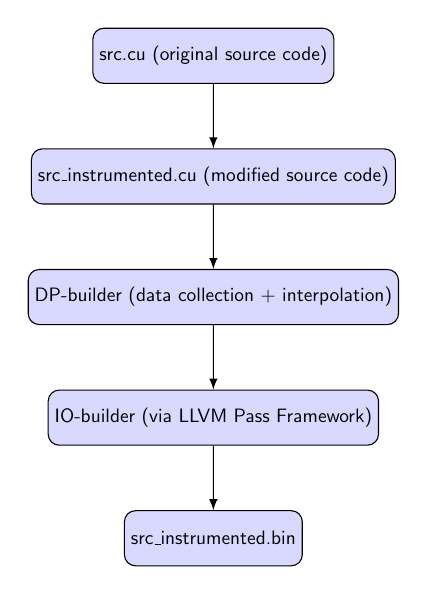
\begin{tikzpicture}[node distance=5cm,
		every node/.style={fill=white, font=\sffamily, scale=0.7}, align=center]
		% Specification of nodes (position, etc.)
		\node (collection)             [process]              {src.cu (original source code)};
		%\node (ifmetric) [ifstatement, below of=curvefitting, yshift=-5em] {\small{Metrics without}\\ \small{Rational Functions?}};
		%\node (dofit) [process, right of=ifmetric, xshift=20em] {Estimate Parameters of\\ Rational Function};
		%\node (encoderatfun) [process, above of=dofit, yshift=0.5em] {Compute Rational Function\\ For Low-Level Metric};
		\node (codegen)      [process, below of=collection,yshift=8em]   {src\_instrumented.cu (modified source code)};
		\node (rateval)     [process, below of=codegen, yshift=8em]   {DP-builder (data collection + interpolation)};
		\node (optimize)      [process,below of=rateval, yshift=8em] {IO-builder (via LLVM Pass Framework)};
		\node (execute)      [process, below of=optimize, yshift=8em] {src\_instrumented.bin};
		\draw[-latex]             (collection) -- (codegen);
		\draw[-latex]      (codegen) -- (rateval);
		\draw[-latex]     (rateval) -- (optimize);
		\draw[-latex]     (optimize) -- (execute);
	\end{tikzpicture}
	%\caption{Generating the rational program ${\cal R}$  when compiling 
		%the multithreaded program ${\cal P}$
		%then using  ${\cal R}$ to optimize the execution of ${\cal P}$. }
\end{figure}
